\documentclass[../thesis.tex]{subfiles}
\graphicspath{{../gfx/}{gfx/}}
\begin{document}
\pagestyle{plain}

\chapter{Wstęp}
\label{intro}

\section{O pracy}

Tematem mojej pracy magisterskiej jest porównanie metod wstępnego przetwarzania i~klasyfikacji danych biomedycznych. Temat ten wydaje mi się ciekawy z wielu powodów.

Podstawowym powodem, dla którego postanowiłem zająć się tym tematem, jest aktualność problemu raka piersi u~kobiet. Zapadalność na raka piersi wzrasta z roku na rok w~krajach wysoko rozwiniętych. W krajach tych, pomimo postępów w~diagnozowaniu i~leczeniu, obserwuje się wzrost corocznej liczby zgonów wywołanej tą chorobą. W Polsce kobiety chorują na raka piersi nieco rzadziej niż w~reszcie świata. U co dwunastej kobiety na świecie diagnozuje się raka piersi, podczas gdy w~Polsce jest to co czternasta kobieta \cite{cancer_web_a}.  Wyleczalność wygląda w~naszym kraju znacznie gorzej. Co druga polka chora na raka piersi umiera z powodu tej choroby, podczas gdy np. w~Holandii jedynie trzy na dziesięć kobiet. Wg badań z 2010 r. nowotwory złośliwe piersi stanowią u~Polek 22\% wszystkich zachorowań nowotworowych \cite{cancer_web_b}.

\begin{figure}[h]
\centering
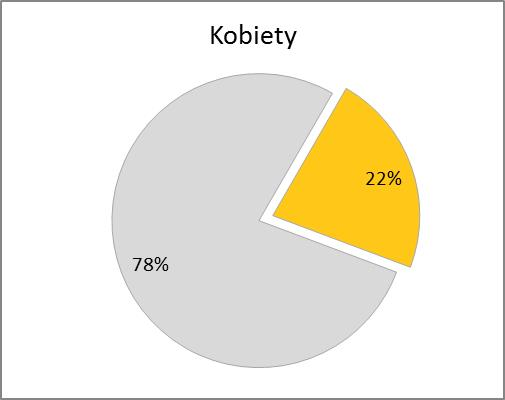
\includegraphics{zachorowalnosc.jpg}
\caption{Częstość zachorowań na nowotwory piersi w~Polsce w~2010 roku}
\label{intro:cancer_chart}
\end{figure}

Drugiem powodem, dla którego postanowiłem zająć się tą pracą, jest popularność metod uczenia maszynowego. Uczenie maszynowe znajduje bardzo wiele praktycznych zastosowań, w~skład których wchodzą: rozpoznawanie obrazów, wyszukiwanie, detekcja spamu, wykrywanie fałszerstw finansowych oraz rozpoznawanie chorób na podstawie symptomów. 

\begin{figure}[h]
\centering
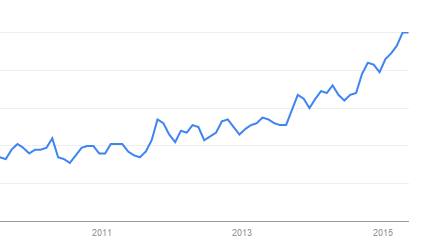
\includegraphics{ml_chart.png}
\caption{Zainteresowanie hasłem \textit{machine learning} wg wyszukiwarki Google Trends}
\label{intro:ml_chart}
\end{figure}

\section{Cel i~zakres pracy}

\subsection{Cel pracy}

Celem mojej pracy magisterskiej jest zaprojektowanie oraz implementacja systemu komputerowego umożliwiającego porównywanie jakości klasyfikacji rozmaitych algorytmów przetwarzania wstępnego i~klasyfikacji danych medycznych. Algorytmy będą badane na danych medycznych. Efektem działania systemu powinien być ranking zbiorów algorytmów, które wprowadził użytkownik. System powinien oferować prosty interfejs użytkownika pozwalający mu na elastyczny wybór rodzin algorytmów do oceny. Część wykonująca obliczenia powinna być możliwie odseparowana od interfejsu, umożliwiając niezależną pracę nad tymi dwoma modułami.

Projekt systemu jest w~pewnym stopniu oparty na danych, jakimi dysponowałem przez cały czas pisania pracy. Dostępne dane są rzeczywiste i~anonimowe, opisują one zachorowalność na raka piersi u~ok. 1000 pacjentek. Zbiór danych posiada sześć kolumn (atrybutów) zawierających informacje o wynikach badań pacjentek oraz kolumnę chorobową (kategorię) określającą, czy pacjentka była chora na nowotwór, czy nie.

\subsection{Zakres pracy}

Zakres mojej pracy można podzielić na część teoretyczną i~praktyczną. Pierwsza z nich obejmuje przede wszystkim wprowadzenie do problemu klasyfikacji danych w~ujęciu uczenia maszynowego, sformułowanie wymagań dotyczących rozwiązania, projekt systemu oraz wnioski z pracy. Druga część koncentruje się na realizacji zaplanowanej architektury, dokładnej specyfikacji niektórych fragmentów implementacji oraz na opisach testów systemu. 

Rozdział następny stanowi wprowadzenie do problemu klasyfikacji oraz przetwarzania wstępnego danych w~kontekście uczenia maszynowego. Po lekturze tego rozdziału czytelnik powinien mieć podstawową wiedzę na temat tego, jak działają algorytmy sztucznej inteligencji użyte w~mojej pracy.

Rozdział trzeci zatytułowany \emph{Założenia i~wymagania systemu} dotyczy wymagań stawianych projektowanemu systemowi obliczeń. Opracowanie wymagań jest bardzo ważnym elementem pracy, ponieważ, poprzez analizę tego co wykonalne, pozwala zrozumieć, jak powinien wyglądać projektowany system. Ze względu na prototypowy typ systemu, praca skupia się na wymaganiach funkcjonalnych i~ograniczeniach narzędziowych oraz implementacyjnych.

Rozdział pt. \emph{Projekt systemu komputerowego} zawiera ideowe opisy modułów programowych użytych w~systemie. W rozdziale tym można znaleźć diagramy klas, opisy funkcji, metod i~architektury systemu. Projekt rozwiązania jest przygotowany niezależnie od późniejszej implementacji, dając autorowi (oraz innym osobom) swobodę w~realizacji systemu.

Rozdział kolejny zatytułowany \emph{Elementy implementacji systemu} pokazuje zasadę działania wybranych, najciekawszych elementów systemu. W części tej znajdują się fragmenty kodu źródłowego wraz z objaśnieniami.

Wyniki badań są zgromadzone w~rozdziale szóstym. Wnioski płynące z analizy wyników badań oraz z całości pracy nad systemem umieszczone są w~ostatnim rozdziale pracy.

\end{document}
